\subsection{Interpretation of Bayesian MLPs}

\begin{figure}[htpb]
    \centering
    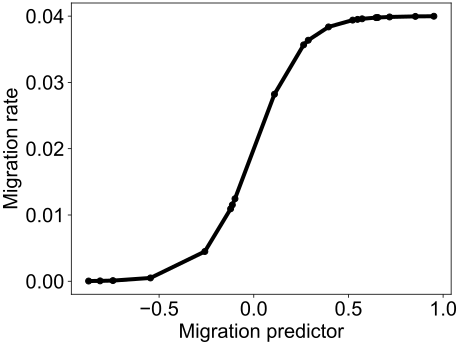
\includegraphics[width=1\textwidth]{figures/epi-multitype.pdf}
    \caption{Results of the MLP-16/8 model for scenario Epi-4, with two continuous predictors—time (relevant, red) and a random predictor (irrelevant, gray). (a) Distributions of partial dependence plots (PDPs) across replicate trees for both predictors. (b) Distributions of SHAP feature importances across trees. (c) Reconstruction of the relationship between the relevant predictor and the inferred migration rates, showing the median estimates across trees with corresponding 95\% credible intervals.}%
    \label{fig:epi-multitype}
\end{figure}

\begin{figure}[htpb]
    \centering
    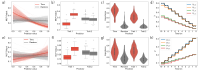
\includegraphics[width=1\textwidth]{figures/fbd-2traits.pdf}
    \caption{Results of the MLP-32/16 model for scenario FBD-4. The analysis includes four predictors: time (relevant, shown in red), a random continuous predictor (irrelevant, gray), and two binary traits: trait~1 (relevant), and trait~2 (irrelevant). The first column shows the distributions of partial dependence plots (PDPs) across replicate trees for the two continuous predictors (time and random). The second column reports PDPs for the two binary traits, where for each violin plot, the left and right halves correspond to trait values of~0 and~1, respectively. The third column presents the distributions of SHAP feature importances across trees. The fourth column displays the median predicted rates through time. The top row refers to the speciation rate (\( \lambda \)), and the bottom row to the extinction rate (\( \mu \)).}%
    \label{fig:fbd-2traits}
\end{figure}

Figure~\ref{fig:epi-multitype} presents the results of the interpretability analyses conducted on the Bayesian MLP models for two distinct inference tasks from the simulation study: estimating migration rates (\( M \)) in scenario Epi-4, and estimating speciation (\( \lambda \)) and extinction (\( \mu \)) rates in scenario FBD-4. The analyses employed partial dependence plots (PDPs) and Shapley values (SHAP).

In scenario Epi-4, the task involved inferring 20 migration rates among five population pairs, using two continuous predictors as MLP inputs. The first predictor was relevant, exhibiting a sigmoidal relationship with the target migration rate, whereas the second was irrelevant, randomly drawn from a uniform distribution. The PDP for the relevant predictor clearly captured the expected sigmoidal trend, while the PDP for the random predictor was essentially flat, indicating no meaningful influence on the model output (Figure~\ref{fig:epi-multitype}a). This pattern was corroborated by the SHAP analysis (Figure~\ref{fig:epi-multitype}b), where the relevant predictor displayed strong feature attribution, and the random predictor contributed negligibly to the predictions.

Scenario FBD-4 focused on estimating speciation (\( \lambda \)) and extinction (\( \mu \)) rates for four classes of species, each defined by combinations of two binary traits. The predictors included time, the two binary traits (one relevant and one irrelevant), and an additional continuous predictor modeled as a random walk with standard normal increments across time bins. For speciation rate predictions, the PDPs with respect to time and the random walk predictor (Figure~\ref{fig:fbd-2traits}a) and with respect to the binary traits (Figure~\ref{fig:fbd-2traits}b) revealed that the MLP effectively captured the decreasing temporal trend and the influence of the relevant trait, while remaining largely insensitive to the irrelevant and random predictors. This interpretation is supported by the SHAP analysis (Figure~\ref{fig:fbd-2traits}c), which identified time and the relevant trait as the most influential features, with the others showing minimal contribution. The median predicted speciation rates across all species classes (Figure~\ref{fig:fbd-2traits}d) further demonstrate that the MLP accurately recovered the distinct evolutionary dynamics associated with each class.

For the extinction rate (\( \mu \)), analogous patterns were observed (Figure~\ref{fig:fbd-2traits}e-h). The PDPs for the relevant trait and time predictor exhibited clear trends, while those for the irrelevant and random predictors remained flat (Figure~\ref{fig:fbd-2traits}e-f). The SHAP values (Figure~\ref{fig:fbd-2traits}g) again highlighted time and the relevant trait as the primary drivers of the model’s predictions, albeit with slightly less pronounced feature attribution than for speciation. Despite this reduced clarity, the MLP successfully produced accurate extinction rate estimates across all populations (Figure~\ref{fig:fbd-2traits}h).
